\section{Data and choice of offices}\label{app:data}

\paragraph{Lapse records.} PATSTAT's legal-event table (INPADOC) records renewal payments, lapses and expiries for
the offices that report them. I scanned every authority for events in the categories ``cessation'', ``maintenance''
and ``payment'' and measured, for granted invention patents filed 2000--2010: the share with a recorded cessation;
the share of 2000--2005 filings whose first cessation comes within 15 years of filing (lapse rather than expiry);
the number of grants with a domestic first applicant; and the years in which cessations are recorded. Event dates
are effective dates unless missing or set to the placeholder 9999-12-31, in which case publication dates are used.
Table~\ref{tab:coverage} summarises the scan. An office is usable if it records cessation for a large share of grants
continuously over the period.

\begin{table}[ht]
\centering
\begin{threeparttable}
\caption{Lapse records in PATSTAT: candidate emerging-market offices}\label{tab:coverage}
\small
% Source: em-patent-value output/coverage_national.csv (22_coverage_scan.py)
\begin{tabular}{lrccrcl}
\toprule
Office & Grants & Cessation & Lapsed by & Domestic & Years & Verdict \\
 & 2000--10 & recorded & 15 years & grants & recorded & \\
\midrule
Russia         & 301{,}160 & 71\% & 74\% & 128{,}782 & 1987--2022 & included \\
Taiwan         & 306{,}085 & 76\% & 53\% & 124{,}228 & 1994--2025 & included \\
Czech Republic &   7{,}413 & 95\% & 62\% &   3{,}196 & 1990--2025 & included \\
Hungary        &   4{,}160 & 66\% & 43\% &   1{,}290 & 1990--2024 & too few firm patents \\
Poland         &  26{,}623 & 34\% & 35\% &  16{,}171 & 1998--2015 & records stop in 2015 \\
Slovakia, Croatia & 2{,}406 / 2{,}254 & 85 / 97\% & 48 / 67\% & 638 / 1{,}000 & & very small \\
\addlinespace
\multicolumn{7}{l}{\emph{No lapse records ($\leq$1\% of grants):} Mexico, South Africa, India, Argentina, Malaysia,
Ukraine,} \\
\multicolumn{7}{l}{\quad Egypt, Colombia, Saudi Arabia, Romania, Bulgaria, Morocco, Peru} \\
\bottomrule
\end{tabular}
\begin{tablenotes}\footnotesize
\item \emph{Notes:} Granted invention patents filed 2000--2010. Lapsed by 15 years: share of 2000--2005 filings whose
first cessation event comes within 15 years of filing. Domestic grants use the raw first-applicant country and are
understated where it is often missing. Inclusion in the analysis also requires about 1{,}000 domestic firm patents
in the 2000--2005 sample; the Czech Republic (909) is kept as a small Central European case, Brazil (164) and Hungary
(299) are dropped. Ten advanced-economy offices pass the same tests; the five largest by domestic firm patents with
full records are used.
\end{tablenotes}
\end{threeparttable}
\end{table}

\paragraph{Advanced-economy offices.} Ten advanced-economy offices have usable records (the United States, Japan,
Germany, the United Kingdom, France, Canada, Australia, Spain, the Netherlands and Sweden). To match the five
emerging-market offices I use the five with the most domestic firm patents.

\begin{figure}[ht]
\centering
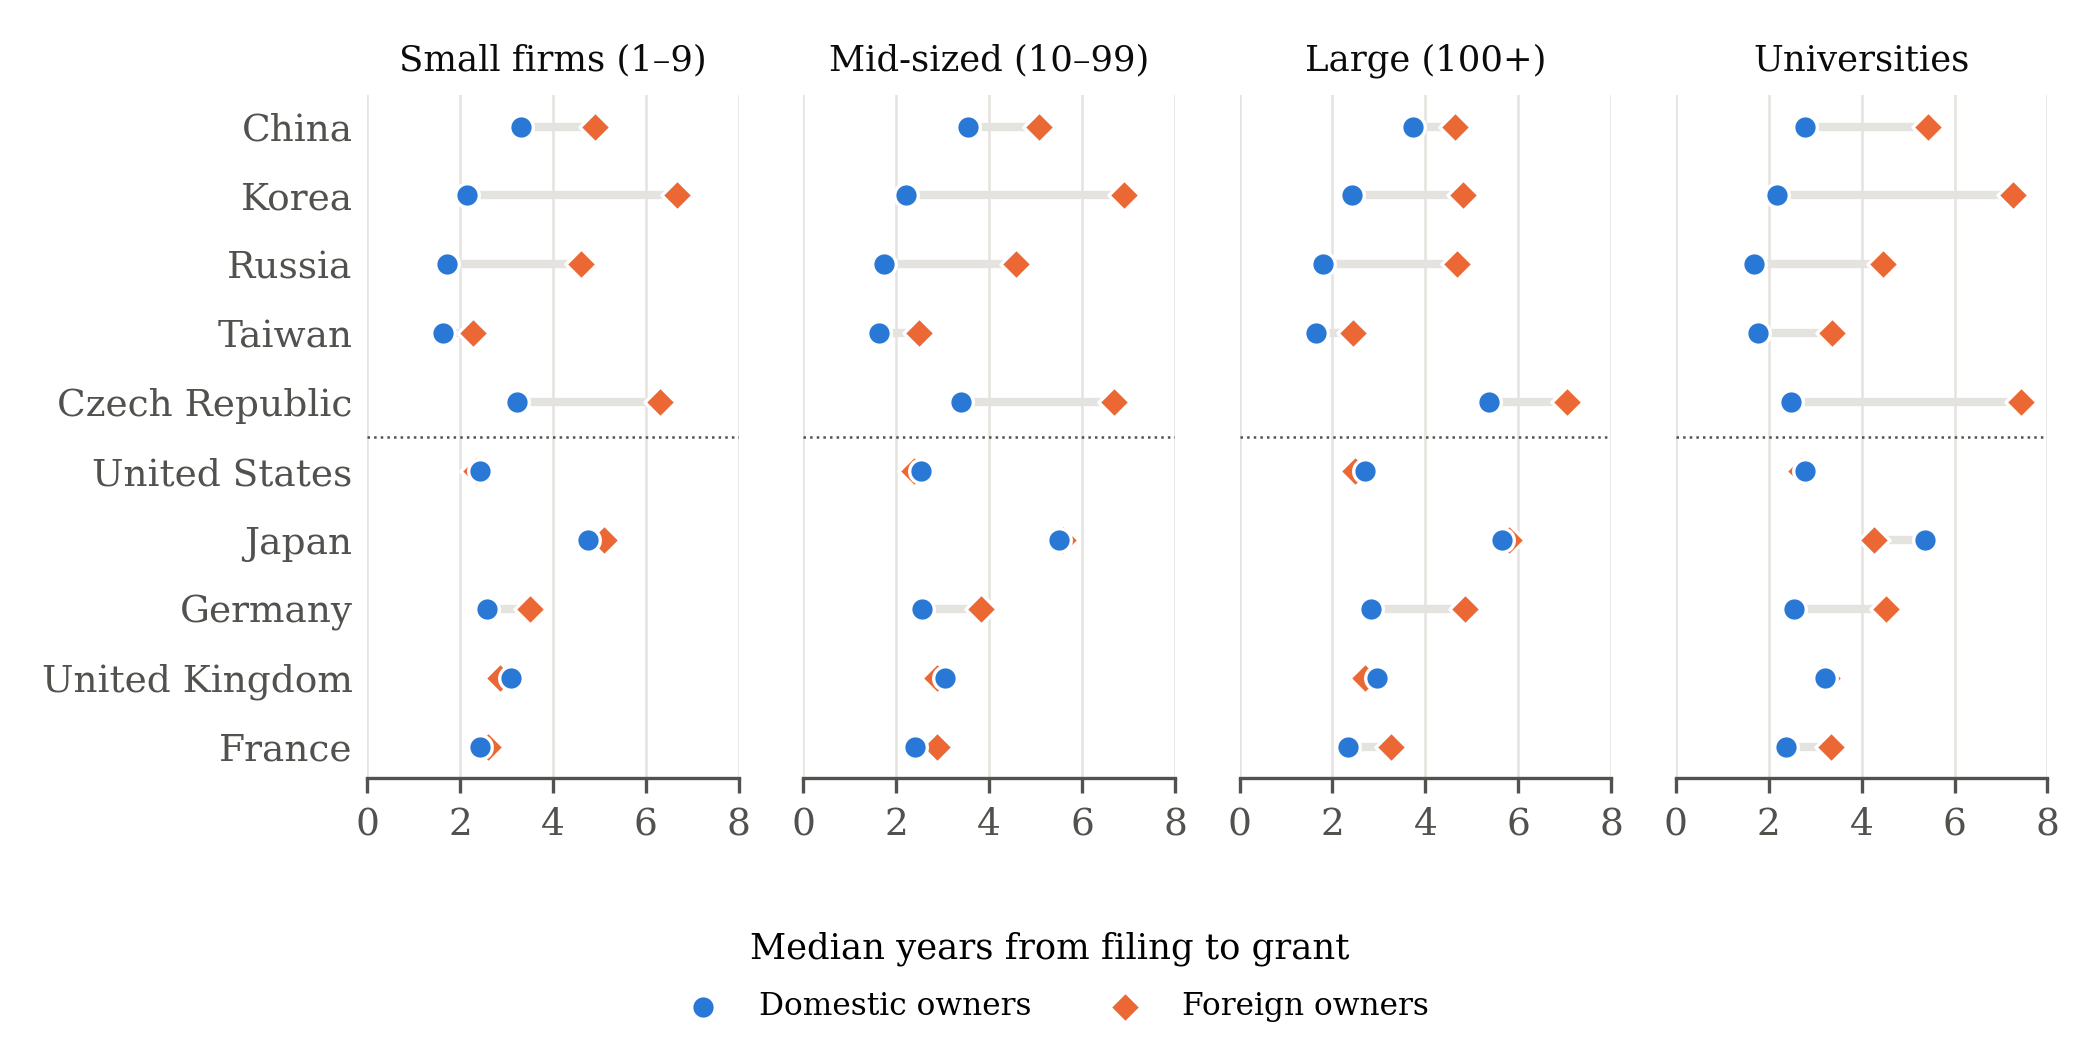
\includegraphics[width=\textwidth]{figures/fig1_grant_lags.png}
\caption{Grant lags by owner and firm size}\label{fig:lags}
\figurenotes{Median years from filing to the first grant publication, patents of Table~1; firm size
as in Table~1. Circles: domestic owners; diamonds: foreign owners. No Czech firm has 100 or more
inventions. Many foreign applications enter through the international (PCT) route, which adds up to 30 months before
national examination begins. Source: em-patent-value output/sample\_lags.csv.}
\end{figure}

\paragraph{Owners and quality.} Owner identities are PATSTAT's harmonised applicant names (HAN). Sector comes from
PATSTAT's sector allocation. Firm size is the number of distinct DOCDB families in which the HAN appears as an
applicant among invention-patent applications filed worldwide in 2000--2005. Applications with no recorded applicant
have no HAN or sector and drop out of the owner-group estimates; they are common among domestic patents in Russia and
foreign patents in Japan and Korea, where national records often omit applicants. Citation counts are citing DOCDB families. Blocking citations are citing applications
whose search report marks the patent X or Y. Grant lag is measured to the first publication flagged as a grant.

\section{Survival: additional results}\label{app:results}

\begin{table}[ht]
\centering
\begin{threeparttable}
\caption{Domestic minus foreign owners within each office, alive 8 years after grant (pp)}\label{tab:within}
\small
% Source: em-patent-value output/ext_within_office_groups.csv (23b_within_office_groups.py; size 2000-2005)
\begin{tabular}{lccccc}
\toprule
 & All owners & Small firms & Mid-sized firms & Large firms & Universities \\
 & & (1--9) & (10--99) & (100+) & \\
\midrule
\multicolumn{6}{l}{\emph{A. Emerging-market offices}} \\
China          & $9.0^{***}$ & $7.2^{***}$ & $13.6^{***}$ & $12.7^{***}$ & $-13.5^{***}$ \\
               & (2.1) & (0.5) & (1.4) & (4.5) & (2.0) \\
Korea          & $12.2^{***}$ & $8.3^{***}$ & $16.7^{***}$ & $11.7^{***}$ & $8.4^{*}$ \\
               & (1.5) & (0.9) & (1.4) & (2.2) & (4.4) \\
Russia         & $-4.2^{**}$ & $-1.1$ & $4.1$ & $-4.1$ & $-8.5^{**}$ \\
               & (1.8) & (1.4) & (4.1) & (8.3) & (4.0) \\
Taiwan         & $15.0^{***}$ & $0.8$ & $9.4^{***}$ & $17.6^{***}$ & $36.6^{***}$ \\
               & (3.1) & (1.3) & (1.9) & (4.4) & (3.5) \\
Czech Republic & $7.7^{**}$ & $9.6^{**}$ & $4.2$ & -- & -- \\
               & (3.2) & (4.8) & (5.5) &  &  \\
\addlinespace
\multicolumn{6}{l}{\emph{B. Advanced-economy offices}} \\
United States  & $2.6^{**}$ & $1.8^{***}$ & $3.4^{***}$ & $2.7^{*}$ & $1.7$ \\
               & (1.1) & (0.3) & (0.4) & (1.6) & (2.6) \\
Japan          & $16.7^{***}$ & $17.8^{***}$ & $20.8^{***}$ & $14.8^{***}$ & $26.0^{***}$ \\
               & (1.8) & (1.1) & (1.3) & (2.5) & (6.5) \\
Germany        & $5.0^{***}$ & $6.1^{***}$ & $1.6$ & $5.7^{**}$ & $5.1$ \\
               & (1.8) & (1.5) & (1.8) & (2.5) & (9.1) \\
United Kingdom & $0.4$ & $2.5^{*}$ & $-0.1$ & $2.4$ & $-13.9^{***}$ \\
               & (1.9) & (1.3) & (2.2) & (6.3) & (3.7) \\
France         & $-1.1$ & $1.7$ & $-0.6$ & $-1.4$ & $1.2$ \\
               & (2.8) & (1.7) & (2.2) & (4.3) & (6.7) \\
\bottomrule
\end{tabular}
\begin{tablenotes}\footnotesize
\item \emph{Notes:} Domestic minus foreign owners, one regression per office and owner group, with log citations,
filing-year and field effects (and owner-group effects for all owners); standard errors clustered by owner in
parentheses. --: fewer than 100 domestic or foreign patents (no Czech firm has 100 or more inventions). $^{*}$~$p<0.1$, $^{**}$~$p<0.05$, $^{***}$~$p<0.01$.
\end{tablenotes}
\end{threeparttable}
\end{table}

\begin{table}[ht]
\centering
\begin{threeparttable}
\caption{Richer quality controls: extra domestic gap in emerging-market offices (pp)}\label{tab:rich}
\small
% Source: em-patent-value output/ext_rich_quality.csv (24_extended_checks.py)
\begin{tabular}{lccc}
\toprule
Owner group & Citations & + blocking, early citations, grant lag & + family size \\
\midrule
Small firms (1--9)       & $2.8^{***}$ & $-0.4$ & $-1.7^{**}$ \\
                         & (0.5) & (0.6) & (0.7) \\
Mid-sized firms (10--99) & $7.9^{***}$ & $5.7^{***}$ & $4.0^{***}$ \\
                         & (0.9) & (1.1) & (1.2) \\
Large firms (100+)       & $9.0^{***}$ & $7.9^{***}$ & $7.8^{***}$ \\
                         & (2.6) & (2.7) & (2.9) \\
Universities             & $-5.7$ & $-5.6$ & $9.6^{**}$ \\
                         & (3.6) & (3.8) & (4.3) \\
\bottomrule
\end{tabular}
\begin{tablenotes}\footnotesize
\item \emph{Notes:} Coefficient $\delta$ of equation~(1) of the paper by owner group, alive 8 years after grant, with
office-specific slopes for each control; standard errors clustered by owner in parentheses. Family size is shown
separately because international filing also reflects owner capacity. $^{*}$~$p<0.1$, $^{**}$~$p<0.05$, $^{***}$~$p<0.01$.
\end{tablenotes}
\end{threeparttable}
\end{table}

\begin{figure}[ht]
\centering
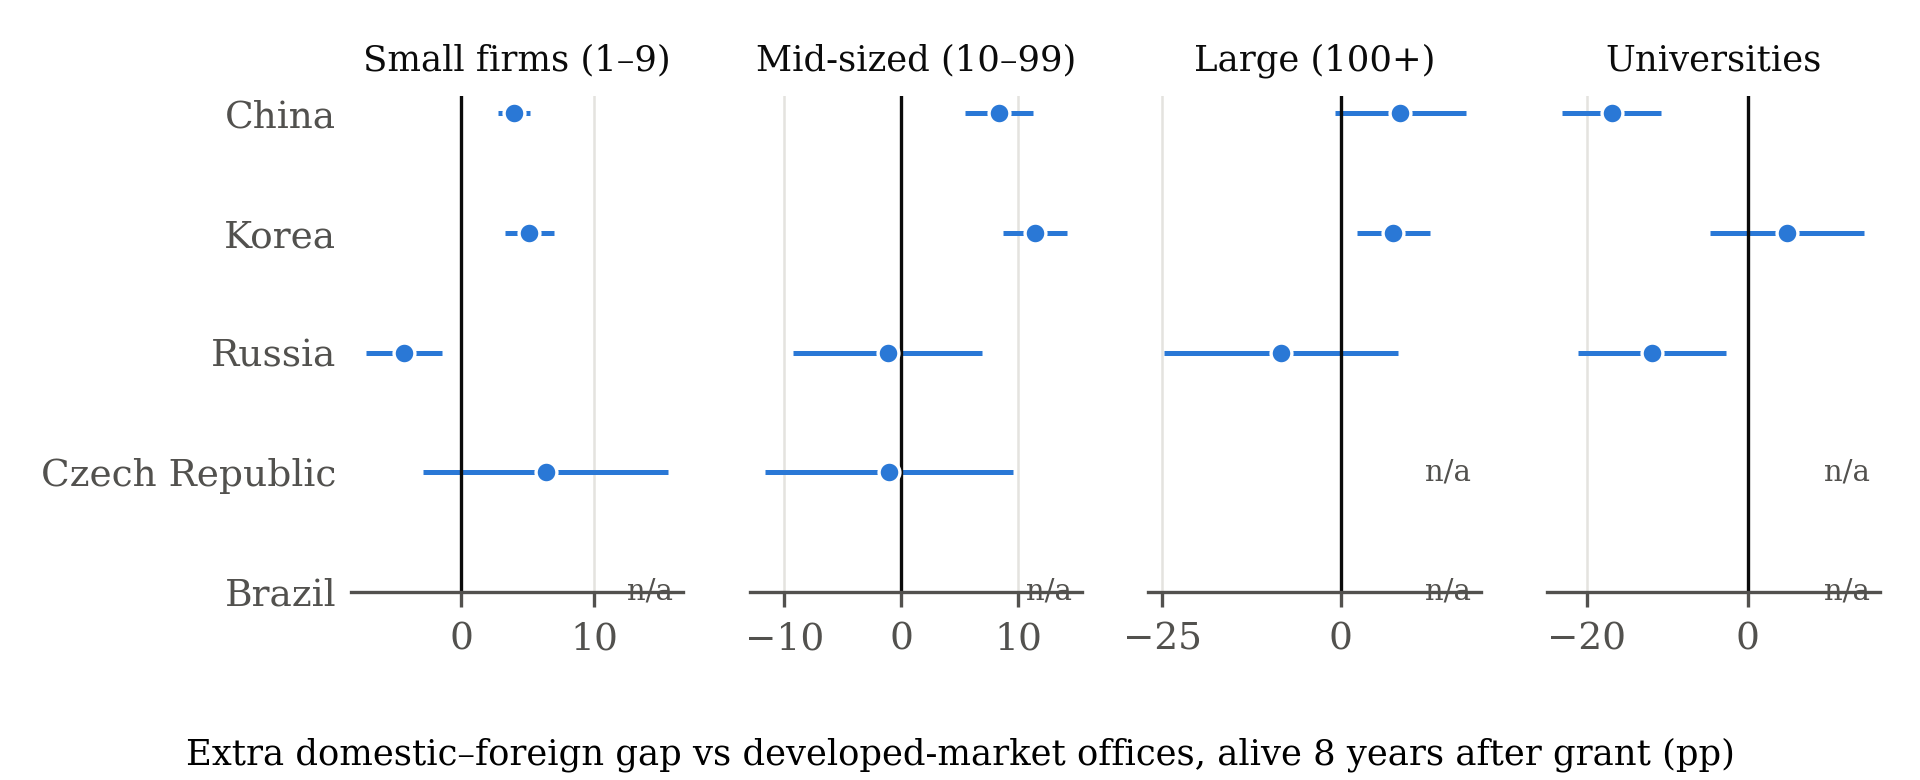
\includegraphics[width=0.95\textwidth]{figures/fig3_by_country.png}
\caption{Each emerging-market office against the advanced-economy offices}\label{fig:country}
\figurenotes{Coefficient $\delta$ of equation~(1) of the paper estimated on one emerging-market office and the five
advanced-economy offices, separately for each owner group, with office $\times$ filing-year and office $\times$ field
effects and office-specific citation slopes; 95\% confidence intervals (standard errors clustered by owner). Outcome:
alive eight years after grant. Firm size: inventions filed worldwide in 2000--2005. n/a: the Czech Republic has no
domestic firm with 100 or more inventions and too few domestic university patents (95).}
\end{figure}

\paragraph{Small against large domestic firms.} A comparison that involves no foreign owners matches domestic small
firms' patents with domestic patents of firms with 100 or more inventions in exact cells of office $\times$ filing year
$\times$ field $\times$ early-citation bin $\times$ blocking-citation bin $\times$ grant-lag bin. Small firms keep their
patents 3.9 points less often than large firms in the advanced-economy offices, and in the emerging-market
offices the difference is the same: the extra gap is 0.6 points. The small-firm shortfall is a small-firm effect,
not an emerging-market one.

\section{Owner constraints: additional results}\label{app:constraints}

\begin{figure}[ht]
\centering
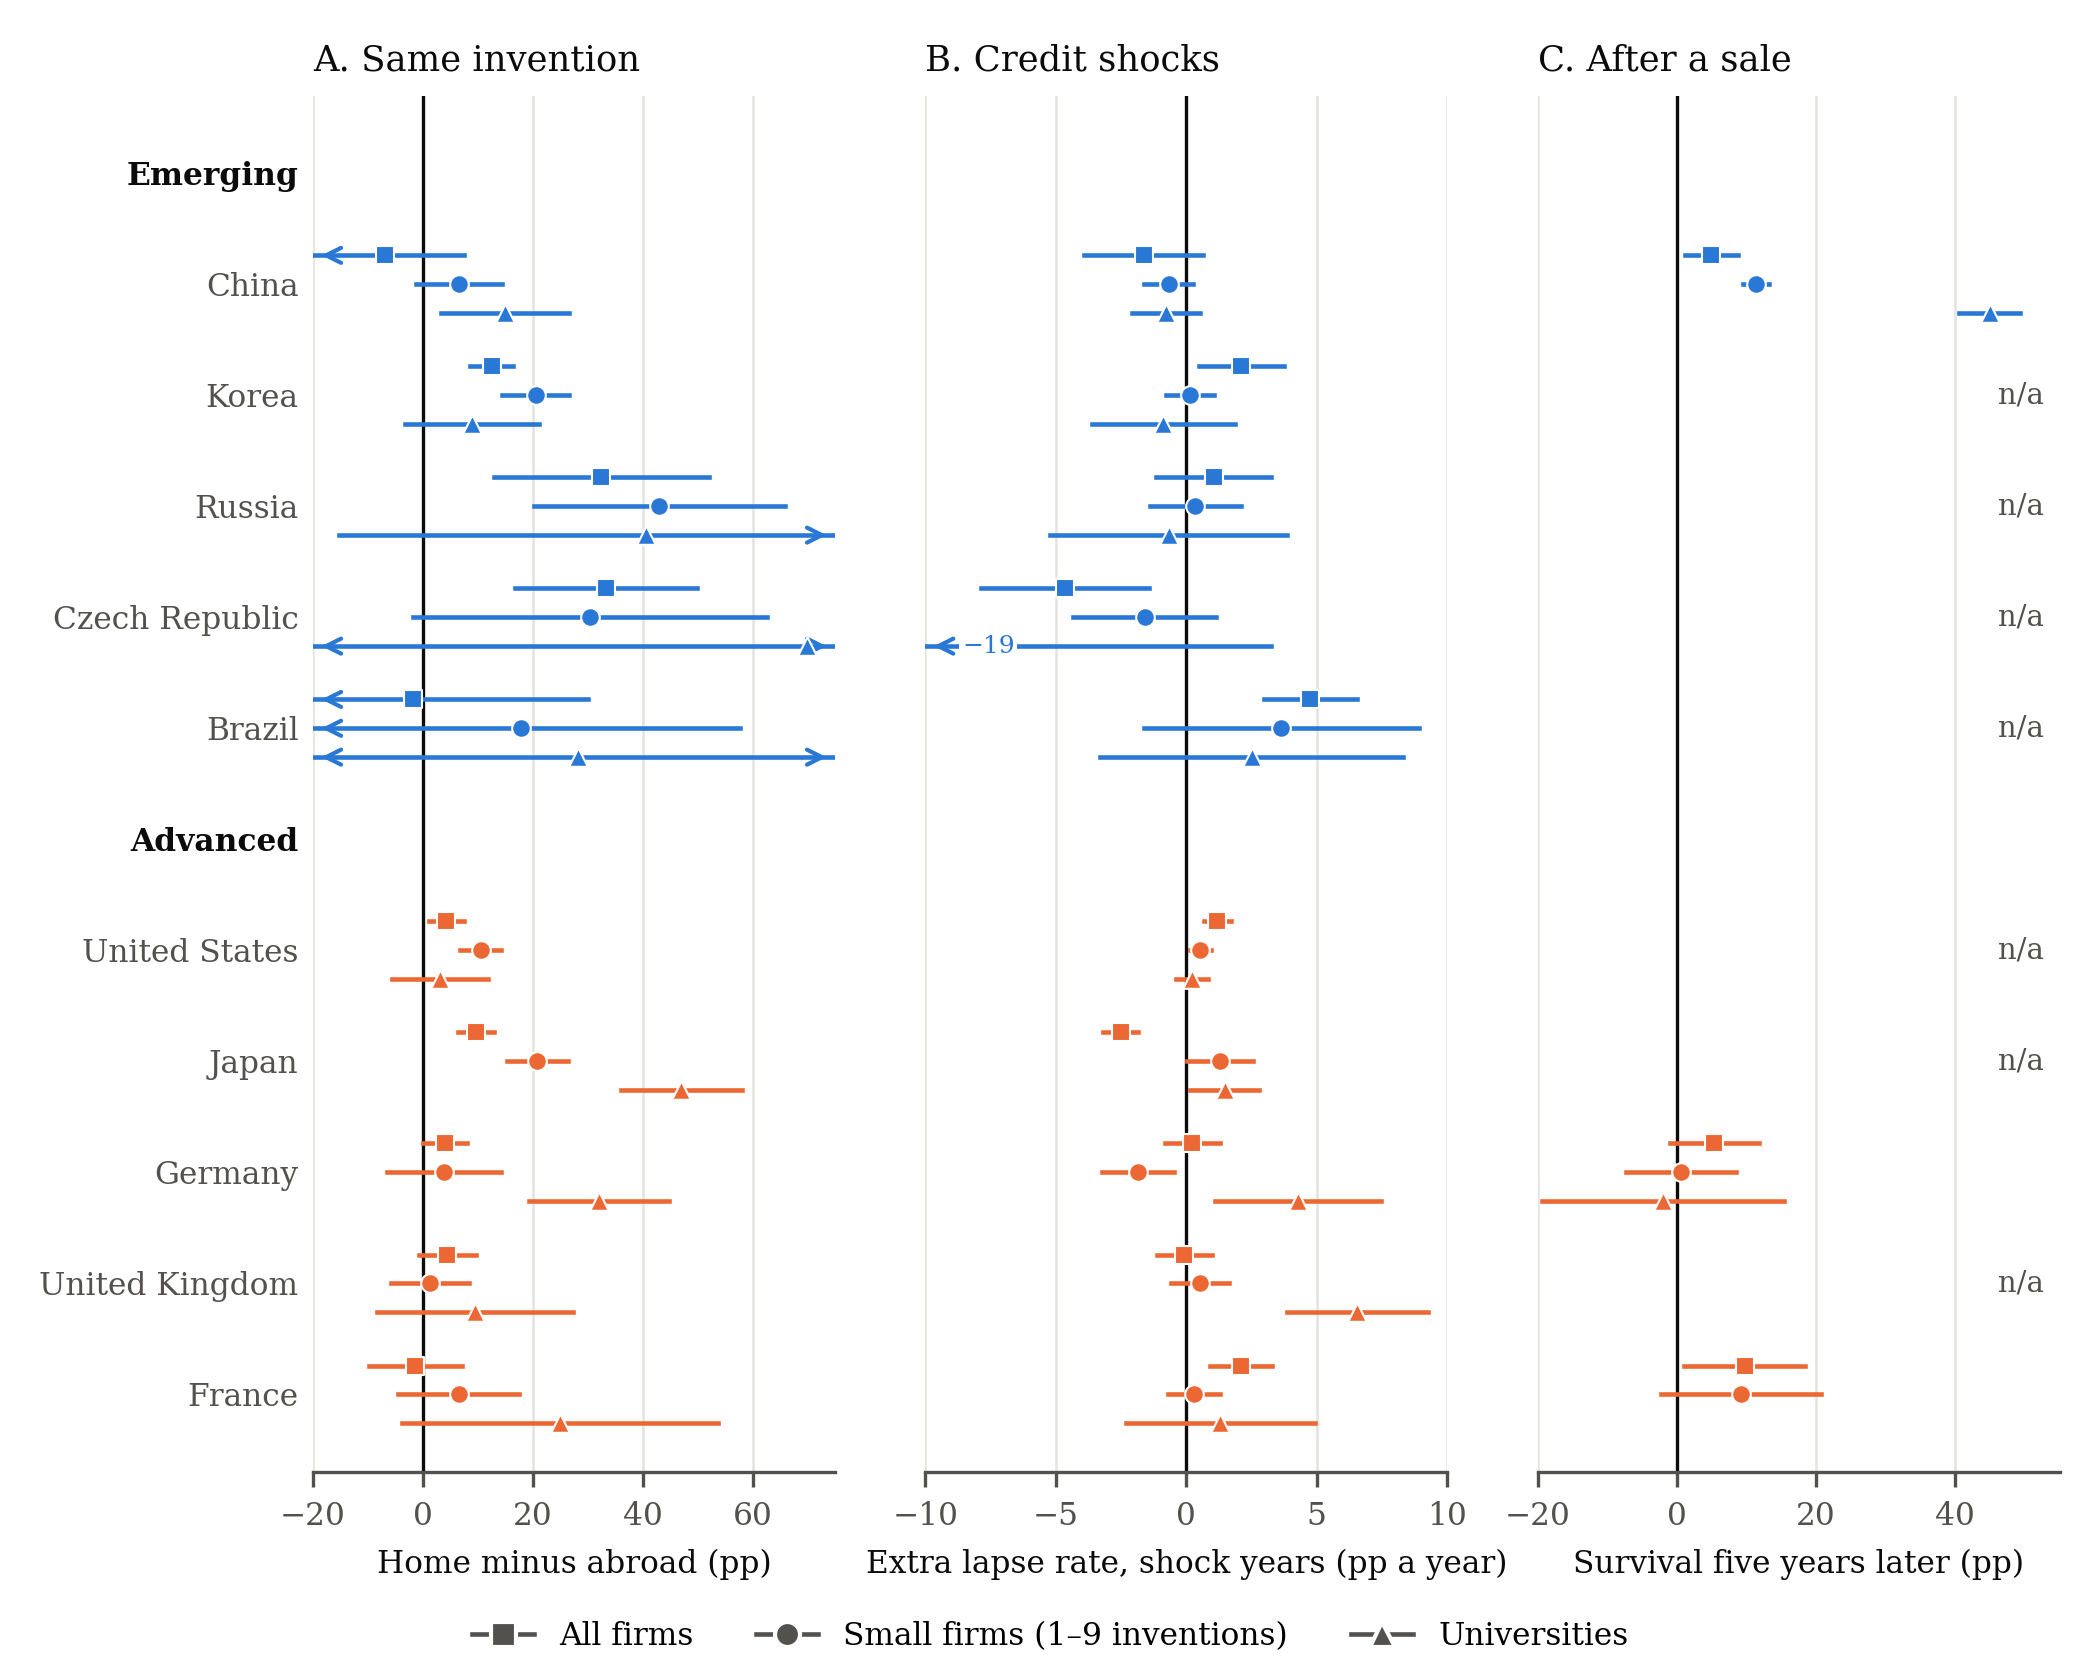
\includegraphics[width=\textwidth]{figures/fig6_constraints_country.png}
\caption{Owner-constraint tests by country}\label{fig:constraints-country}
\figurenotes{Point estimates with 95\% confidence intervals, in percentage points; blue: emerging economies, orange: advanced economies; squares: all firms, circles: small firms (1--9 inventions filed worldwide in 2000--2005), triangles: universities. Arrows: interval beyond the axis; a number replaces a point beyond it. The estimates of Figure~1 by country of origin (A) or office (B, C), specified as in footnote~3. n/a: no sales of granted patents recorded (Korea records changes of owner only before grant).}
\end{figure}

\begin{table}[ht]
\centering
\begin{threeparttable}
\caption{Responses of small firms to fee changes}\label{tab:fees}
\small
% Source: em-patent-value output/fee_response.csv (17_fee_response.py; size 2000-2005)
\begin{tabular}{@{}l>{\raggedright\arraybackslash}p{0.42\textwidth}cc@{}}
\toprule
Office & Variation & Coefficient & Elasticity \\
\midrule
China & 85\% discount window extended (2016, 2018), intent to treat & 0.0017 (0.0004) & 0.05 \\
Korea & 30\%/50\% discounts for years 4+ (2014, 2016, 2018) & $-0.033$ (0.027) & n.i. \\
United States & stage-specific fee changes (2004, 2013, 2020) & 0.047 (0.019) & 0.26 \\
\quad placebo: 100+ firms & stage-specific fee changes & 0.009 (0.048) & 0.05 \\
United States & 2022 small-entity discount (50\% to 60\%) & 0.023 (0.024) & -- \\
France & SME reductions for years 2--7 (2005, 2008), intent to treat & $-0.083$ (0.027) & n.i. \\
\bottomrule
\end{tabular}
\begin{tablenotes}\footnotesize
\item \emph{Notes:} n.i.: not identified. Panel of renewal decisions of small firms (1--9 inventions filed worldwide in 2000--2005); outcome:
the patent lapses at that payment. Regressor: log of the fee or fee multiplier the owner faces; controls are firms with
100 or more inventions, which are not eligible. Korean lapse records end in 2019, so only the 2014--2018 windows identify the Korean discounts. The French
estimate has the wrong sign and keeps it with small-firm $\times$ filing-cohort effects ($-0.100$, 0.033); it is not
read as an elasticity. Eligibility in France depends on employment (under 250, then 1{,}000 employees), which patent
counts measure only roughly.
\end{tablenotes}
\end{threeparttable}
\end{table}

\section{Renewal models and patent values}\label{app:models}

The deterministic and learning models are set out in Appendix~A of the paper.

\paragraph{Fees.} Fee schedules by year of life and period come from official sources for each office (laws,
decrees, fee regulations and office notices), with the basis of each fee: per year from filing (China, Germany, the
United Kingdom), per year from registration with a per-claim component (Korea, Japan, with ten claims assumed), three maintenance payments at 3.5, 7.5 and 11.5 years after grant (United States, with small-entity fees for firms
with fewer than 100 families and universities), per year from filing from year 3 (Russia, where foreign owners paid
a separate non-resident schedule until August 2012, in US dollars before 2009, converted at the year's exchange
rate), per year from filing from year 2 (France) or year 1 (Czech Republic, where years 1--5 were prepaid at grant
before July 2002), or per year from the grant announcement (Taiwan, whose 2002 schedule is assumed for 2000--2001). Fees are converted to 2024 PPP dollars with the consumer price index
of the year paid (for Taiwan, the DGBAS index and the IMF implied PPP rate); fees due after 2024 are held at 2024
prices. Russian lapse records end in 2022, so Russian patents are censored from mid-2022.

\paragraph{Fee discounts.} For the bounds in Section~5, eligible owners are domestic firms with 1--99
families and domestic universities. In China they pay 40\% of the fee in fee-years 1--3 from the grant year (to
February 2001), 30\% in fee-years 1--3 (to August 2016), 15\% in fee-years 1--6 (to July 2018) and 15\% in fee-years
1--10 (from August 2018). In Korea, registration fees for years 1--3 fall outside the model; owners pay 70\% of the
fee in years 4--6 from March 2014 and 50\% in years 4 and later from April 2018.

\begin{table}[ht]
\centering
\begin{threeparttable}
\caption{Learning model: rate of decline and fit}\label{tab:learning}
\small
% Source: em-patent-value output/learning_model_params*.csv, learning_model_fit*.csv (20_learning_model.py)
\begin{tabular}{lcccccccccc}
\toprule
 & CN & KR & RU & TW & CZ & US & JP & DE & GB & FR \\
\midrule
Free estimate of $d$        & 0.47\tnote{a} & 0.67\tnote{a} & 0.95\tnote{a} & 0.93 & 0.58\tnote{a} & 0.47\tnote{a} & 0.73\tnote{a} & 0.851 & 0.840 & 0.834 \\
$\sigma_0$ at $d = 0.85$    & 1.13 & 1.35 & 7.39\tnote{a} & 2.14 & 1.92 & 2.64 & 2.91 & 1.53 & 1.89 & 1.74 \\
Shock $s$                   & 0.99 & 0.64 & 1.39 & 1.06 & 1.21 & 0.34 & 0.99 & 1.01 & 1.03 & 1.16 \\
Learning $\varphi$          & 0.95 & 0.99 & 0.94 & 0.99 & 0.72 & 0.99 & 0.99 & 0.86 & 0.83 & 0.89 \\
Fit error (pp)              & 2.7 & 3.7 & 6.5 & 3.3 & 2.9 & 1.6 & 2.9 & 2.3 & 2.3 & 2.5 \\
\bottomrule
\end{tabular}
\begin{tablenotes}\footnotesize
\item \emph{Notes:} Fit error: predicted minus observed share alive at 4, 8 and 12 years after grant, by owner group.
\item[a] Not identified: the estimate comes with an implausibly wide spread of initial values.
\item The other rows are estimated with $d = 0.85$ fixed in every office. Taiwan's free estimate rests on fees that
rise in three-year steps; its reported standard error (0.002), like the others, understates the uncertainty.
\end{tablenotes}
\end{threeparttable}
\end{table}

\begin{table}[ht]
\centering
\begin{threeparttable}
\caption{Patent-level values, domestic minus foreign owners, by office (log points)}\label{tab:patentvalues}
\small
% Source: em-patent-value output/patent_value_gaps*.csv (21_patent_values.py, 21b_value_gaps_all_owners.py)
\begin{tabular}{lccccc}
\toprule
 & All owners & Small firms & Mid-sized firms & Large firms & Universities \\
 & & (1--9) & (10--99) & (100+) & \\
\midrule
\multicolumn{6}{l}{\emph{A. Emerging-market offices}} \\
China          & $0.25^{***}$ & $0.20^{***}$ & $0.40^{***}$ & $0.40^{**}$ & $-0.83^{***}$ \\
               & (0.08) & (0.03) & (0.06) & (0.18) & (0.07) \\
Korea          & $0.34^{***}$ & $0.49^{***}$ & $0.87^{***}$ & $0.14$ & $0.47^{**}$ \\
               & (0.08) & (0.06) & (0.07) & (0.11) & (0.19) \\
Russia\tnote{a}& -- & $-0.20$ & $1.75^{**}$ & $2.21$ & -- \\
               &  & (0.63) & (0.74) & (1.95) &  \\
Taiwan         & $0.84^{***}$ & $-0.07$ & $0.33^{***}$ & $1.09^{***}$ & $1.75^{***}$ \\
               & (0.19) & (0.08) & (0.11) & (0.27) & (0.32) \\
Czech Republic & $-0.04$ & $0.07$ & $-0.18$ & -- & $-0.16$ \\
               & (0.16) & (0.20) & (0.23) &  & (0.57) \\
\addlinespace
\multicolumn{6}{l}{\emph{B. Advanced-economy offices}} \\
United States  & $0.34^{***}$ & $0.23^{***}$ & $0.45^{***}$ & $0.41^{***}$ & $0.13$ \\
               & (0.05) & (0.02) & (0.03) & (0.12) & (0.20) \\
Japan          & $1.14^{***}$ & $1.22^{***}$ & $1.52^{***}$ & $0.91^{***}$ & $2.07^{***}$ \\
               & (0.10) & (0.07) & (0.09) & (0.16) & (0.58) \\
Germany        & $0.01$ & $0.20^{***}$ & $-0.02$ & $-0.01$ & $-0.18$ \\
               & (0.07) & (0.06) & (0.07) & (0.10) & (0.33) \\
United Kingdom & $0.06$ & $0.08$ & $0.03$ & $0.20$ & $-0.59^{***}$ \\
               & (0.08) & (0.06) & (0.09) & (0.26) & (0.15) \\
France         & $-0.04$ & $0.00$ & $0.06$ & $-0.06$ & $-0.48^{*}$ \\
               & (0.09) & (0.07) & (0.09) & (0.14) & (0.27) \\
\bottomrule
\end{tabular}
\begin{tablenotes}\footnotesize
\item \emph{Notes:} Posterior median value at grant of each patent from the learning model with a common prior
($d=0.85$; 2024 PPP dollars), regressed on domestic owner $\times$ owner group with fee-path $\times$ citation-band and
field effects, one regression per office (all owners: domestic owner with owner-group effects); standard errors
clustered by owner in parentheses. 1.42 million patents. --: too few patents. Japanese university estimates are
unstable across specifications. $^{*}$~$p<0.1$, $^{**}$~$p<0.05$, $^{***}$~$p<0.01$.
\item[a] Not identified (Section~5); domestic ownership is collinear with the fee path for all owners,
and there are no foreign university patents in the Russian estimation sample.
\end{tablenotes}
\end{threeparttable}
\end{table}

\clearpage
\newpage 

\section{Returns at stake in the learning model}\label{app:leverslearning}

Table~\ref{tab:levers-learning} repeats Table~3 with the learning model ($d=0.85$). Each patent's
returns follow the model's random walk, and owners renew while the expected returns of keeping the patent, including
the option of later renewals, exceed the fee; a lever therefore also changes the value of that option. Markets for technology are calibrated to the
same survival gains as in Table~3; the factors are 1.54 for small firms, 1.52 for mid-sized firms and
21 for universities, against 1.41, 1.39 and 5.0 in the deterministic model. Levels are about ten times those of
Table~3 for markets for technology and five times for university patenting; fee relief is still worth
about a million dollars a cohort, so the ranking of the levers is unchanged.

\begin{table}[ht]
\centering
\begin{threeparttable}
\caption{Returns at stake per filing-year cohort, learning model (millions of 2024 PPP dollars)}\label{tab:levers-learning}
\small
% Source: em-patent-value output/policy_levers_learning.csv (26b_policy_levers_learning.py)
\begin{tabular}{lcccc}
\toprule
 & \multicolumn{2}{c}{Fee relief} & Markets for technology & University patenting \\
\cmidrule(lr){2-3}\cmidrule(lr){4-4}\cmidrule(lr){5-5}
 & China & Korea & China & China \\
\midrule
Small firms (1--9)          & 0.12 & 0.4 & 1{,}250 &  \\
Mid-sized firms (10--99)    & 0.05 & 0.3 & 992 &  \\
Large firms (100+)          & n.e. & n.e. & 0 &  \\
Universities                & 0.4  & 0.3 & 8{,}390 & 982--1{,}413 \\
\addlinespace
All owners                  & 0.6  & 0.9 & 10{,}633 & 982--1{,}413 \\
\quad \% of national R\&D   & 0.00 & 0.00 & 11.30 & 1.04--1.50 \\
\bottomrule
\end{tabular}
\begin{tablenotes}\footnotesize
\item \emph{Notes:} As Table~3, with the learning model: 3{,}000 patents per owner group drawn from the
estimation cells, 200 return paths each. n.e.: not eligible.
\end{tablenotes}
\end{threeparttable}
\end{table}
